% Senseigigs — how a gig becomes a provider shortlist.
% Standalone slide figure. Compile: pdflatex -interaction=nonstopmode senseigigs_arch.tex
% Render: pymupdf page.get_pixmap(dpi=300) -> .png -> .jpg  (no pdftoppm/convert here)
%
% Design (glance test): ONE spine, 4 numbered stages left->right, plain-English labels.
% No file names, formulas or index internals. The gig's own text is carried through.
%
% Layout notes, all from LOOKING at a render (estimates were wrong every time):
%  - step numbers are INLINE in the headings. Circle badges collided with the centred
%    heading of the longest card (rendered as "R<badge>ank the best 50").
%  - the title sets \sffamily EXPLICITLY: a node-level font= REPLACES the picture's
%    \sffamily instead of inheriting it, which rendered the title in serif.
%  - headings are short enough to fit ONE line at this text width; when any wraps to
%    two lines its body starts lower and the row of cards loses its shared baseline.
%  - every card body is exactly two lines.
%  - the tile row is centred on x=0 (4 x 39mm + 3 x 4mm = 168mm, so it starts at -84mm
%    and t1's CENTRE is at -64.5mm) and the caption is centred on the row via calc.
%  - the bbox is symmetric, so the centred title is centred on the page too.
\documentclass[border=12pt]{standalone}
\usepackage[T1]{fontenc}
\usepackage{tikz}
\usetikzlibrary{arrows.meta, positioning, fit, backgrounds, calc}
\usepackage{amssymb}

\definecolor{gigC}{HTML}{2B6CB0}
\definecolor{searchC}{HTML}{2F855A}
\definecolor{rankC}{HTML}{C05621}
\definecolor{outC}{HTML}{6B46C1}
\definecolor{inkC}{HTML}{2D3748}

% small italic footer line inside a card
\newcommand{\sub}[1]{{\footnotesize\itshape\color{inkC}#1}}

\begin{document}
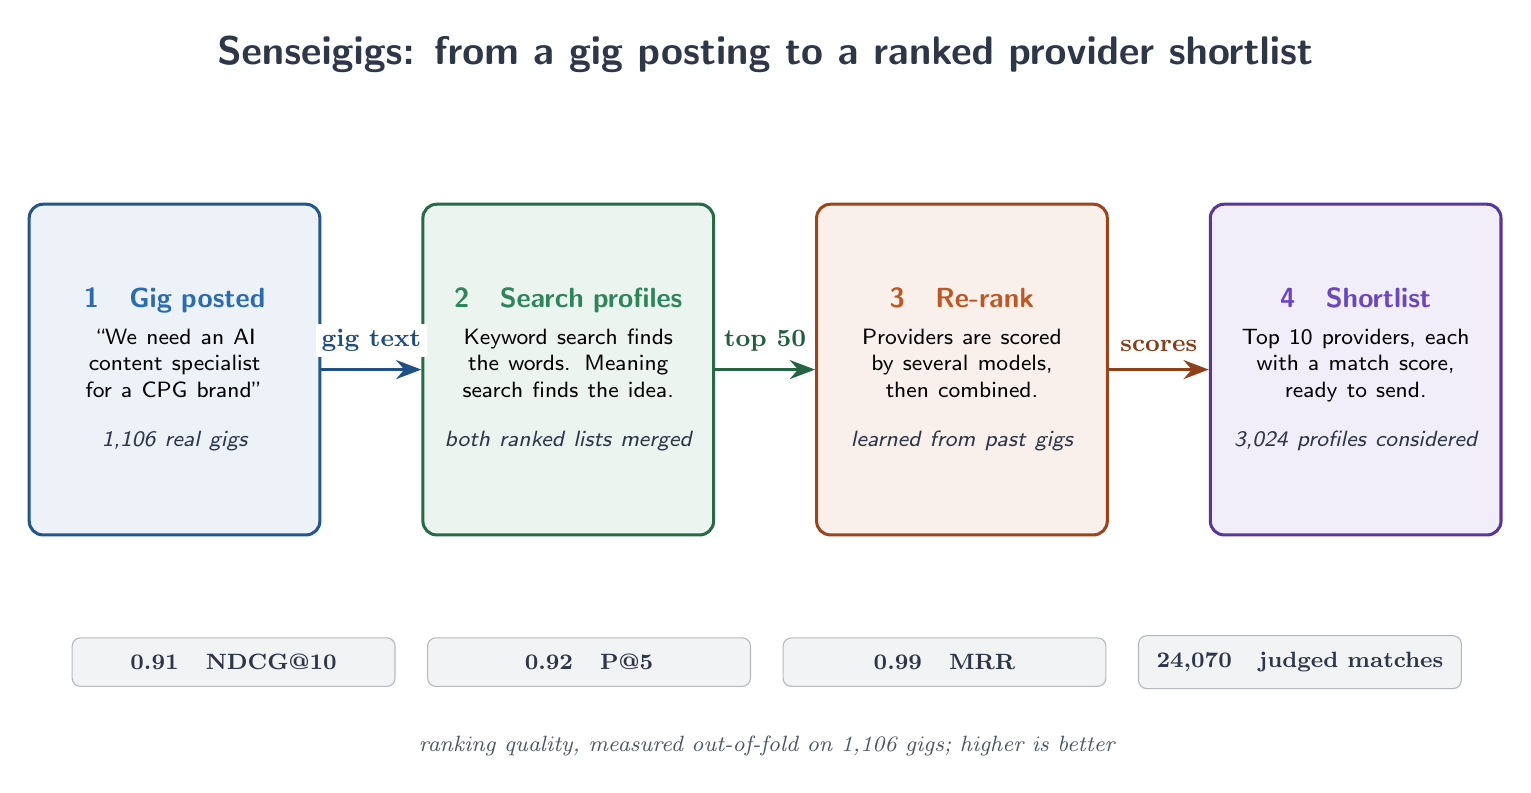
\begin{tikzpicture}[
  font=\sffamily,
  every node/.style={align=center},
  card/.style={rounded corners=5pt, draw=#1!80!black, fill=#1!9, line width=1.1pt,
               inner sep=7pt, text width=32mm, minimum height=42mm},
  flow/.style={-{Stealth[length=3.2mm,width=2.4mm]}, line width=1.3pt, draw=#1!75!black},
  flowlab/.style={font=\small\bfseries, text=#1!70!black, fill=white, inner sep=2pt},
  tile/.style={rounded corners=3pt, draw=inkC!35, fill=inkC!6, inner sep=6pt,
               font=\footnotesize, text=inkC, minimum width=41mm},
]

% ---------------- title ----------------
\node[font=\sffamily\Large\bfseries, text=inkC] (title) at (0,4mm)
  {Senseigigs: from a gig posting to a ranked provider shortlist};

% ---------------- the four stages ----------------
\node[card=gigC] (s1) at (-75mm,-36mm) {%
  {\color{gigC}\bfseries 1\quad Gig posted}\\[4pt]
  \footnotesize ``We need an AI content
  specialist for a CPG brand''\\[6pt]
  \sub{1{,}106 real gigs}};

\node[card=searchC] (s2) at (-25mm,-36mm) {%
  {\color{searchC}\bfseries 2\quad Search profiles}\\[4pt]
  \footnotesize Keyword search finds the words.
  Meaning search finds the idea.\\[6pt]
  \sub{both ranked lists merged}};

\node[card=rankC] (s3) at (25mm,-36mm) {%
  {\color{rankC}\bfseries 3\quad Re-rank}\\[4pt]
  \footnotesize Providers are scored\\
  by several models,\\
  then combined.\\[6pt]
  \sub{learned from past gigs}};

\node[card=outC] (s4) at (75mm,-36mm) {%
  {\color{outC}\bfseries 4\quad Shortlist}\\[4pt]
  \footnotesize Top 10 providers, each\\
  with a match score,\\
  ready to send.\\[6pt]
  \sub{3{,}024 profiles considered}};

% ---------------- the flow ----------------
\draw[flow=gigC]    (s1.east) -- node[flowlab=gigC, above, yshift=1.4mm] {gig text} (s2.west);
\draw[flow=searchC] (s2.east) -- node[flowlab=searchC, above, yshift=1.4mm] {top 50} (s3.west);
\draw[flow=rankC]   (s3.east) -- node[flowlab=rankC, above, yshift=1.4mm] {scores} (s4.west);

% ---------------- evidence tiles: equal width, centred on the spine ----------------
% 4 x 41mm + 3 x 4mm = 176mm, so the row starts at -88mm and t1's CENTRE is at -67.5mm.
\node[tile, anchor=north] (t1) at (-67.5mm,-70mm) {\bfseries 0.91\quad NDCG@10};
\node[tile, right=4mm of t1] (t2) {\bfseries 0.92\quad P@5};
\node[tile, right=4mm of t2] (t3) {\bfseries 0.99\quad MRR};
\node[tile, right=4mm of t3] (t4) {\bfseries 24{,}070\quad judged matches};

\coordinate (rowC) at ($(t2.south)!0.5!(t3.south)$);
\node[font=\footnotesize\itshape, text=inkC!85, anchor=north] (cap)
  at ([yshift=-5mm]rowC) {ranking quality, measured out-of-fold on 1{,}106 gigs; higher is better};

\end{tikzpicture}
\end{document}
